\section{Системийн судалгаа}
Сонгосон сэдэв болох ``Ажил олгогчдын өгөгдлийн анализ систем дээр суурилсан чатбот'' сэдвийн хүрээнд судалгаа хийхдээ чатбот системийн талаар болон өгөгдөл цуглуулгын аргын талаар судалсан. Үүний дараа ижил төстэй системийн болон ашиглагдах технологийн талаар судалгааг хийсэн болно.
\subsection{Чатбот систем}
Чатбот систем нь ихэвчлэн хэрэглэгчийн асуултыг хиймэл оюун ухааны тусламжтайгаар ойлгож, хариултыг автоматжуулах үндсэн зорилготой компьютерийн програм хангамж юм. Орчин үед хэрэглэгчдэд туслах үндсэн үүргийн дагуу чатбот системийг байгууллагууд олон янзаар ашиглах болсон. Тэдгээрээс дурдвал,
\begin{itemize}
  \item Цэс дээр суурилсан чатбот (Menu-based chatbot)
  \item Түлхүүр үгийг танихад суурилсан чатбот (Keyword recognition-based chatbot)
  \item Машин сургалтын чатбот (Machine learning chatbot)
\end{itemize}
\textbf{Цэс дээр суурилсан чатбот}
\\Өнөөгийн зах зээлд хэрэгжиж буй чатботуудын хамгийн энгийн бөгөөд түгээмэл хэлбэр юм.\cite{chatbotsystem} \footnote{\url{https://www.engati.com/blog/types-of-chatbots-and-their-applications}} Хэрэглэгчийн асууж болох асуултуудыг урьдаас таамаглан хариултуудыг мод хэлбэртэйгээр бүтэцлэн хадгалдаг. Хэрэглэгч хүссэн хариултаа авахын тулд системийн хадгалсан хариултаар аялах хэрэгтэй болдог. Бусад чатботтой харьцуулбал, хариулт хязгаарлагдмал бөгөөд хэрэглэгчээс олон асуулт асууж цаг их шаарддагаараа сул талтай байдаг. 
\\
\textbf{Түлхүүр үгийг танихад суурилсан чатбот}
\\Энэхүү чатбот нь хэрэглэгчийн бичсэнийг уншиж тохиромжтой хариултыг өгдөг. Ингэхдээ өгүүлбэрийг хиймэл оюун ухааны нэг хэсэг болох эх хэлний боловсруулалт (Natural Language Processing)-ын тусламжтайгаар шинжилж түлхүүр үгийг таньж хариултыг өгдөг. Ижил төстэй олон асуултад хариулах эсвэл түлхүүр үг дутуу үед амжилтгүй болдог. Мөн хэрэглэгч хүссэн хариултаа олж чадахгүй байх болон үр дүн муутай хариулт өгсөн тохиолдолд цэс дээр суурилсан чатботыг хослуулан ашиглах нь найдвартай болдог бөгөөд түгээмэл шийдлүүдийн нэг байдаг. 
\\
\textbf{Машин сургалтын чатбот}
\\Энэ төрлийн чатбот нь өмнө хэрэглэгчийн харилцан яриан дээр хиймэл оюун ухаан болон машин сургалтын тусламжтайгаар шинжилгээ хийж, хэрэглэгчийн зан төлөв, асуултын хэв маягаас суралцдаг. Ингэснээрээ чатботод хэрэглэгчийн зарцуулах цаг эрчимтэйгээр буурах буюу хариултаа авах алхам багасгах ба хэрэглэгчийн туршлага (UX) нь түүнийгээ даган өсөх нь энэхүү чатботын үндсэн зорилго болно. 
\\
\textbf{Чатботыг сонгох}
\\Машин сургалтын чатбот нь илүү уян хатан хэрэглэгчдэд ээлтэй чатботыг бий болгодог боловч хөгжүүлэхэд цаг хугацаа их шаардагдах ба машин өөрөө суралцахад мөн хугацаа шаардагддаг. Иймд системийн нөөц, шаардлагыг харгалзан үзэж энэхүү судалгааны ажлаар түлхүүр үг танихад суурилсан чатботыг хэрэгжүүлэхийг зориод байна. 
\subsection{Өгөгдөл цуглуулгын арга}
Өгөгдөл цуглуулах (data scraping) нь хэрэглэгчдэд харагдаж буй өгөгдлийг олон янзын сувгаас цуглуулан хувийн орчинд хадгалан цаашид ашиглах боломжийг олгодог хамгийн үр дүнтэй автомат өгөгдөл олборлох арга юм. Ихэвчлэн өгөгдөл цуглуулах арга нь вэбсайтаас шаардлагатай өгөгдлийг цуглуулахад ашигладаг. Өгөгдөл цуглуулж буй хүнээс хамааран олборлосон өгөгдлийг таслалаар тусгаарлагдсан утгын (Comma-Separated Values) файл эсвэл өгөгдлийн санд хадгалах боломжтой бөгөөд нэгэнт цуглуулсан их хэмжээний өгөгдөлд судалгаа шинжилгээ хийх, худалдаа, борлуулалтын хэрэгсэл болгох зэрэг олон төрлийн боломжийг олгодог. 
\\ Вебсайтаас өгөгдлийг олборлох хамгийн түгээмэл арга нь HTML parsing буюу HTML-ийг задлан шинжлэх юм. Энэ нь вебсайтын HTML болох сайтын үндсэн бүтцийг агуулгынх нь хамтаар хуулах бөгөөд авах гэж буй өгөгдлийн зан төрхийг нь зааж өгснөөр доторх агуулгыг хамгийн хялбар бөгөөд автомат байдлаар цуглуулдаг юм. 
Цуглуулга хийх 2 үндсэн арга байдаг. Үүнд:
\begin{itemize}
  \item Өгөгдлийг цуглуулж, задлах (Data scraping)
  \item Өгөгдлийг олж илрүүлж, хаягийг цуглуулах (Data crawling)
\end{itemize}
\textbf{Өгөгдлийг цуглуулж, задлах}
\\Нэг үгээр хэлбэл өгөгдлийг цуглуулж, задлах нь зааж өгсөн хаягийн дагуу шаардлагатай өгөгдлийг задалж, хэрэгтэй агуулгыг хөгжүүлэгчдэд өгдөг бөгөөд хүссэн өгөгдлөө задлан авах боломжийг олгодгоороо давуу талтай. Өөрөөр хэлбэл өгөгдөл олборлох програм нь зорилго буюу даалгавраа мэдэж байгаа юм. 
\\\textbf{Өгөгдлийг олж илрүүлж, хаягийг цуглуулах}
\\Энэхүү аргачлал нь хаяг тодорхой бус үед түүнийг олж илрүүлж шаардлагын дагуу хаягийг, зарим тохиолдолд өгөгдлийг цуглуулдаг. Системийн шаардлагын дагуу өгөгдлийг цуглуулах үед хаяг алгасах, дутуу өгөгдөл цуглуулахаас сэргийлдэг давуу талтай. 
\\Ихэвчлэн энэхүү хоёр аргыг хослуулан ашигладаг бөгөөд шаардлагад нийцэх өгөгдлийг үлдээлгүй бүгдийг нь олоход \textit{data crawling}-ийг ашиглах бол олсон өгөгдлийг задалж, шинжлэн өгөгдлийн санд хадгалах үйлдлийг \textit{data scraping} хийдэг. Жишээлбэл, худалдааны сайтын бараа бүтээгдэхүүний өгөгдлийг цуглуулах гэж байгаа гэж үзвэл, барааны ангиллын хаягуудыг өөрчлөгдөх бүрд хадгалан өгөгдлийг цуглуулна. Өөрөөр хэлбэл нэг нь өөрчлөлт гарахыг ажиглаж вебсайтаар мөлхөж байх бол нөгөө нь шаардлагын дагуу бүх хэрэгтэй өгөгдлийг хэдийн цуглуулсан байна.  
Энэхүү бакалаврын судалгааны ажлын хүрээнд өгөгдлийг CSV файл үүсгэн хадгалж цаашид ашигласан болно. 
\section{Ижил төстэй системүүд}
Гадаад ба дотоодын байгууллагуудын үйл ажиллагаандаа хэрэгжүүлдэг чатбот системүүдээс, \textit{Domino's Pizza \& Pizza Hut} болон {WHO's Chat bot} гэсэн гурван чатботыг сонгон авч судалгаанд оруулав. 
\subsection{Domino's Pizza \& Pizza Hut}
Domino's pizza хоолны газар нь захиалгын алхмаас эхлээд бүх мэдээллийг ганцхан \textit{Facebook messenger chatbot} хангадаг. Чатбот эрчээ авч эхэлсэн шалтгаан нь хүмүүс, бусад хүмүүсийг хүлээлгүйгээр үйлчилгээ авах, тусламж авах зэрэг үйлчилгээг зэрэг нэвтрүүлсэнтэй холбоотой билээ. Үүний нэгэн адилаар Монголд үйл ажиллагаа явуулж буй Pizza Hut Mongolia юм.
\begin{figure}[ht]
  \centering
  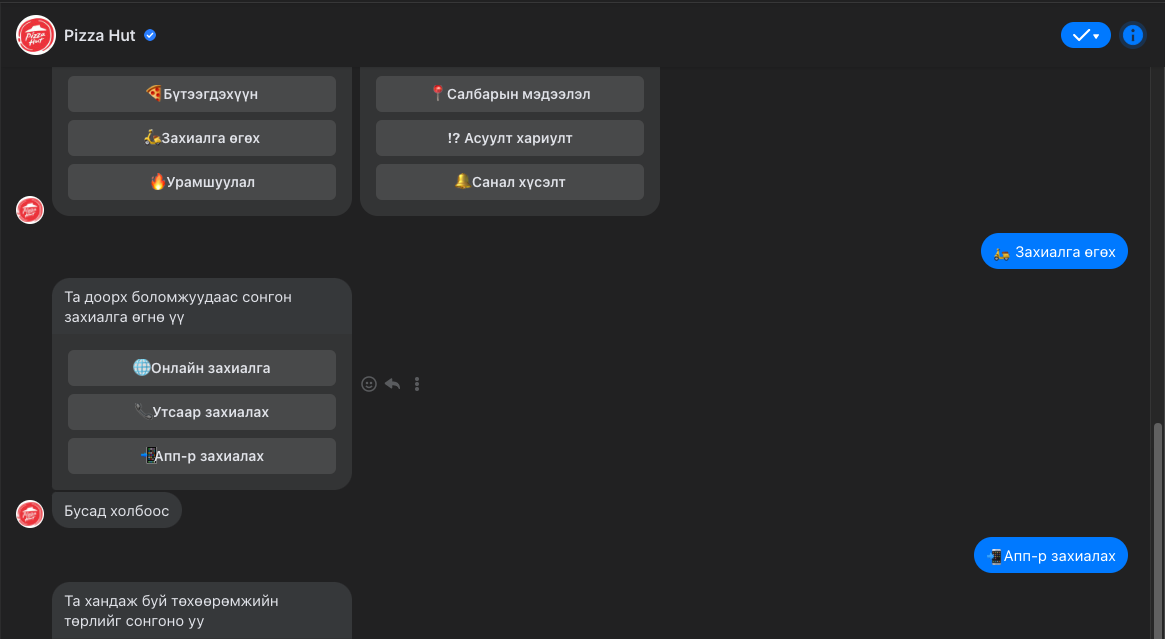
\includegraphics[width=\textwidth]{images/pizzaHut.png}
  \caption{Pizza Hut chat bot}\label{fig:chatbotPizzahut}
\end{figure}
\\Үйлчлүүлэгчдийн захиалга хүлээх хугацааг багасгахын тулд захиалгын үйл явцыг хурдасгаснаар тодорхой хэмжээнд нөлөөлж байгаа нь дээрх 2 жишээнээс харагдаж байна.

\subsection{World Health Orgazination's Chat bot}
Цар тахал болох коронавирусын эрчимтэй тархаж байх үед дэлхийн өнцөг булан бүрд оршин суугаа хүмүүст цар тахлын мэдээлэл, урьдчилан сэргийлэх арга, баталгаатай эх сурвалжийн мэдээллээр хангах зорилготой чатбот юм.
Дэлхий нийтээр вакцинжуулалтын хөдөлгөөн өрнөж байх үеэр вакцины талаарх мэдээлэл, архаг хууч өвчинд нөлөөлөх талаар найдвартай, хамгийн сүүлийн үеийн албан ёсны мэдээллийг өгдөг. Хэдий халдварын тоо буурч, нийгэм өөрөө дасан зохицож байгаа хэдий ч Дэлхийн Эрүүл Мэндийн байгууллага үүргээ гүйцэтгэж чухал эх сурвалжаар хангасаар байгаагийн шинж юм. 
\begin{figure}[ht]
  \centering
  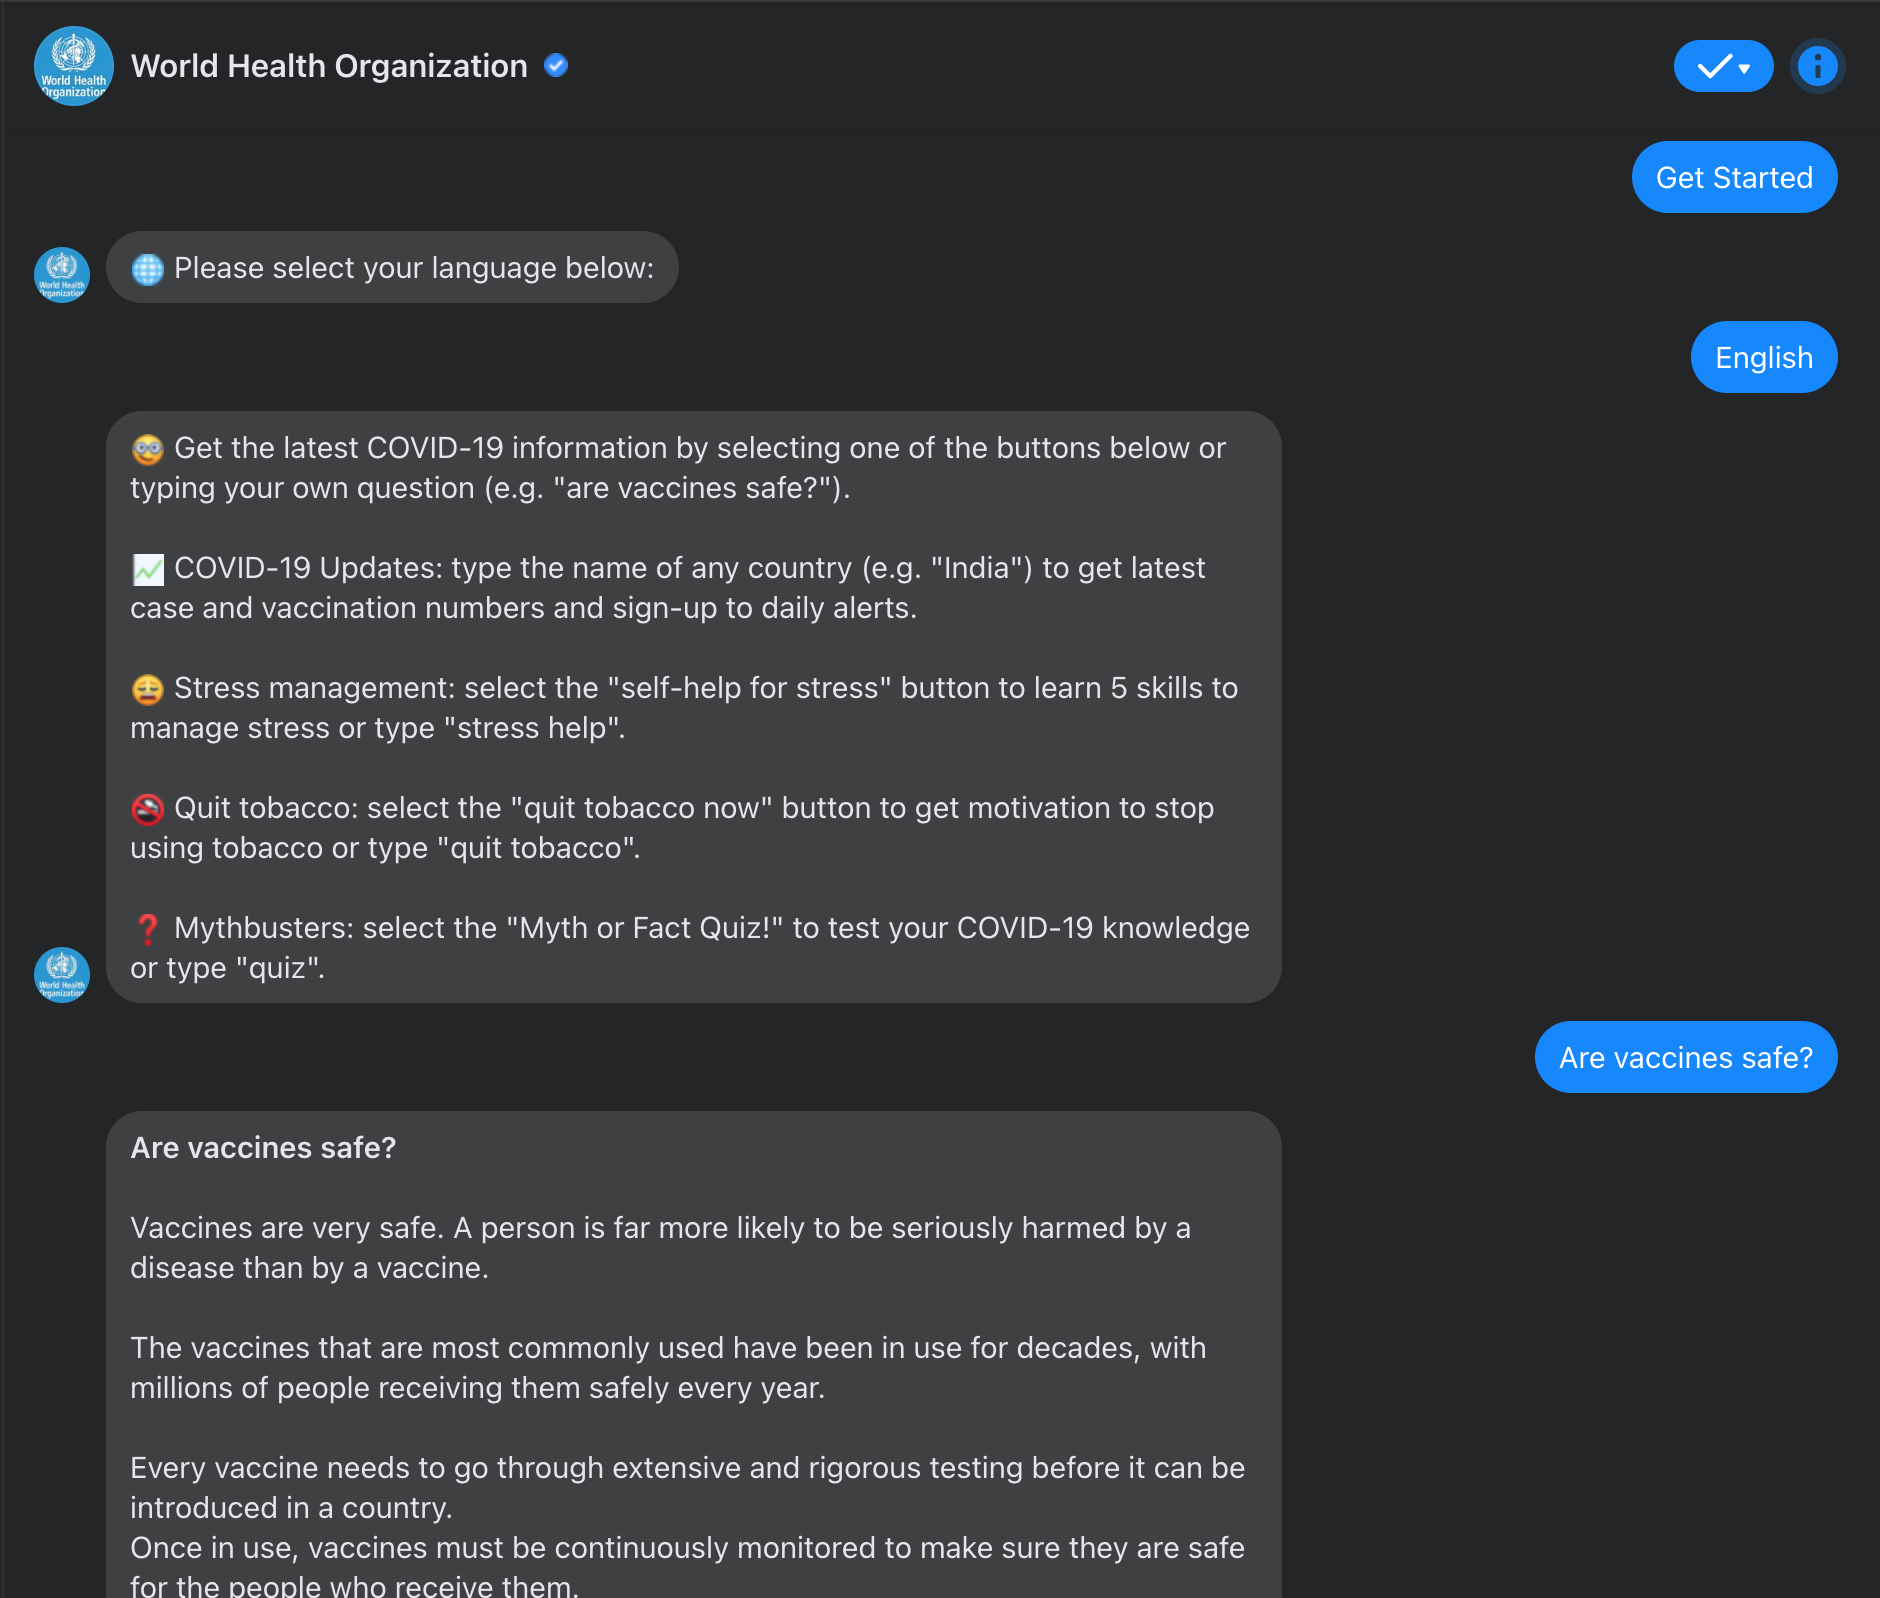
\includegraphics[width=\textwidth-4cm]{images/whoBOT.png}
  \caption{WHO's chat bot}\label{fig:chatbotWHO}
\end{figure}
\section{Технологийн судалгаа}
\@title-ыг хөгжүүлэхдээ өгөгдөл цуглуулгыг \textit{python} хэлний сан болох \textit{BeautifulSoup} HTML өгөгдөл задлах технологийг ашигласан бөгөөд чатбот системийн түлхүүр үг таних технологийг \textit{Python} хэлний \textit{Framework} болох \textit{SentenceTransformers}-ийг сонгон хөгжүүлэлтийг хийсэн. Харин цуглуулсан өгөгдлийг \textit{CSV} файлд хадгалан, \textit{Microsoft Bot Framework}-ийг чатбот хөгжүүлэлтэд ашиглан судалгааг дараах байдлаар хийсэн болно. 
\subsection{Python}
Python нь дээд түвшний маш олон төрлийн програмчлалыг өөртөө шингээсэн хэл юм. Хэлний сан болон \textit{framework}-үүд нь тасралтгүй сайжирч, шинэчлэгдэж байдаг тул бүх л төрлийн програмчлалын аргуудыг гүйцэтгэж болдог. Орчин үед машин сургалт, хиймэл оюун ухаан болон эх хэлний боловсруулалтад(NLP) түгээмэл ашигладаг болсон бөгөөд веб хүртэл хийх боломжтойгоороо давуу талтай юм. Үүнээс гадна анхлан суралцаж буй хүмүүст ойлгоход хялбар \textit{syntax}-ийн дүрэмтэй байдаг тул хэрэглэгчдийн тоо нь javascript, java хэлүүдтэй өрсөлдөхүйц байдаг. 
\begin{figure}[ht]
  \centering
  
\includegraphics[width=4.5cm]{images/pythonLogo.png}
  \caption{Python лого}\label{fig:pythonLogo}
\end{figure}
\lstinputlisting[language=Python, caption=Python энгийн жишээ]{code/pythonTest.py}
Python програмчлалын хэл нь ойлгоход маш хялбар бөгөөд өөр дээрх функцууд нь шууд утгаараа ойлгомжтой байдаг. Syntax-ийн хувьд ; ашигладаггүй ба догол мөрөөр програмчлалын үндсэн схемийг гаргадгаараа онцлог хэл юм.
\subsection{BeautifulSoup}
Өгөгдөл цуглуулгын олон технологиудын нэг нь \textit{BeautifulSoup} бөгөөд \textit{python} програмчлалын хэлний сан юм. Энэ нь өгсөн вебсайтын хаяг (Url)-ийн дагуу бүх HTML өгөгдлийг агуулгын хамтаар нь хэрэглэгчид өгдөг. HTML хэл нь мод хэлбэртэй байдаг бөгөөд түүний хүүхэд элементүүдийн агуулгыг шаардлага болон түлхүүр үгийн дагуу цуглуулах зарчмаар ажилладаг. 
\begin{figure}[ht]
	\centering
  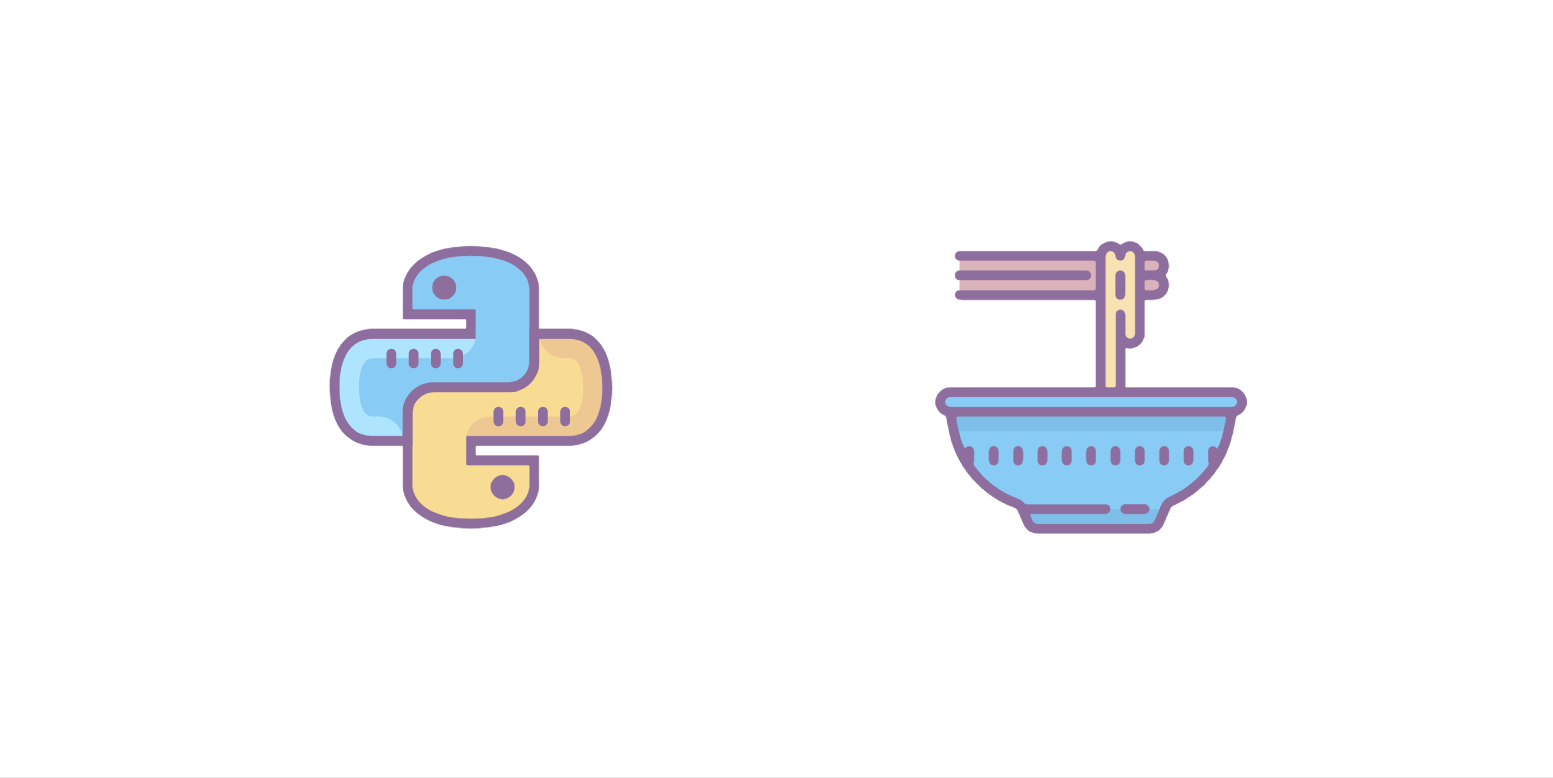
\includegraphics[height=4.5cm]{images/bs4.png}
	\caption{BeautifulSoup лого}\label{fig:bsLogo}
\end{figure}
\\Бакалаврын судалгааны ажлын сэдвийн дагуу ажлын байр олгогчдын мэдээлэл болон ажлын байрны мэдээллийг \textbf{zangia.mn}-ээс \textit{BeautifulSoup} ашиглан цуглуулсан. Доорх кодын жишээнд бүх ажлын байрны ангилал болон шүүлтүүрийн агуулгыг цуглуулсан бөгөөд жишээнд зориулж зөвхөн эхний ангиллын мэдээллийг харуулав.
\lstinputlisting[language=Python, caption=BeautifulSoup жишээ өгөгдөл цугуулалт]{code/bs.py}
\begin{figure}[ht]
  \centering
  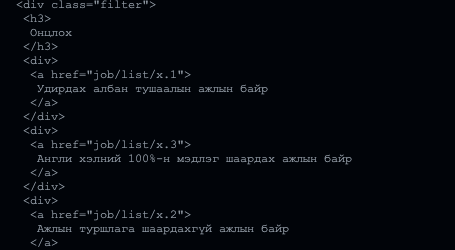
\includegraphics[height=5.5cm]{images/bsExample.png}
	\caption{Өгөгдөл цуглуулалтын жишээний үр дүн}\label{fig:resultBS}
\end{figure}
\subsection{SentenceTransformers}
Python хэлний framework болох SentenceTransformers \cite{sentenceTransform} буюу өгүүлбэр хувиргалт нь өгүүлбэр болон текстийн ижил төстэй байдал болон утгын хувьд адил байдлыг \textit{cosine-similarity}\footnote{Cosine-similarity нь өгөгдлийн шинжилгээнд 2 тооны ижил төстэй байдлыг вектор үржвэрээр илэрхийлдэг.}-ийн тусламжтайгаар тооцоолдог. Энэхүү тооцооллыг цаашид өгүүлбэрийн ижил төстэй байдлыг харьцуулах, хайлт хийх, түүнд шинжилгээ хийх зэргээр ашиглаж болно. Доорх зурагт өгүүлбэрт хувиргалт хийж, шинжилгээний үр дүнгийн вектор хоорондын өнцгөөр хэрхэн тодорхойлогддог болох талаар харуулав.
\begin{figure}[ht]
  \centering
  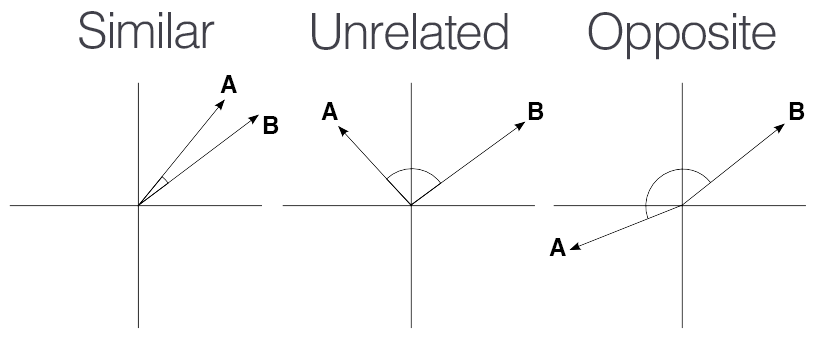
\includegraphics[height=5cm]{images/cosineSimilarity.png}
  \caption{Cosine similarity утгын график}\label{fig:cosineSimilarity}
\end{figure}
\\SentenceTransformers-ийг дэлхийн 100 гаруй хэл дээр урьдчилан бэлтгэн, сургасан эх хэлний боловсруулалт (NLP)-ын загваруудыг ашиглаж болдгоороо давуу талтай.
\begin{figure}[ht]
  \centering 
  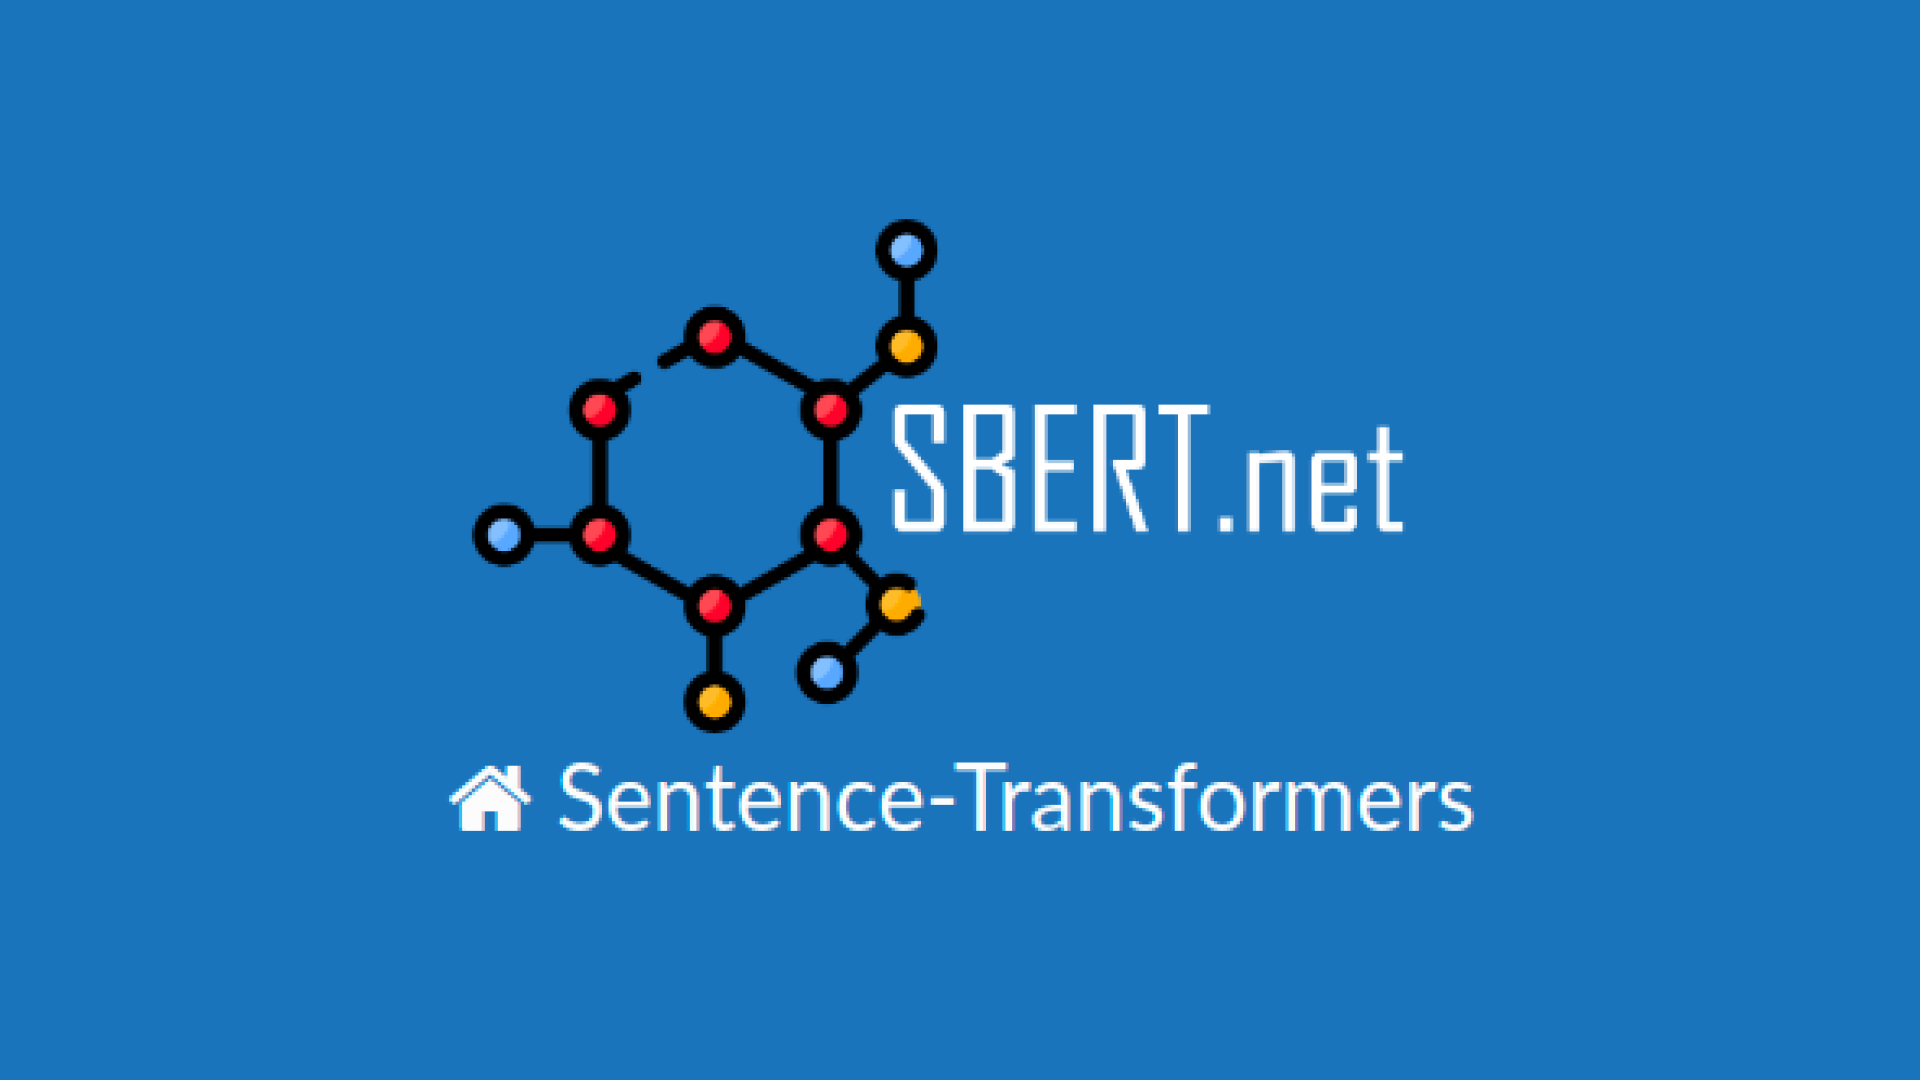
\includegraphics[height=5cm]{images/sbertLogo.png}
  \caption{SBERT.net лого}\label{fig:sbertLogo}
\end{figure}
\\Чатбот системийн хувьд монгол хэлийг танин ашиглах боломжтой загвар болох \textit{distiluse-base-multilingual-cased-v2}\cite{sbert}-ийг ашиглан хийж гүйцэтгэв.
\\Хоёр өгүүлбэрийг \textit{cosine-similarity} ашиглан ижил төстэй байдлыг илэрхийлэх жишээг доор харууллаа. Эх кодыг utf-8 формат танихгүй байсан тул зураг хэлбэрээр орууллаа.
\\
\begin{figure}[ht]
  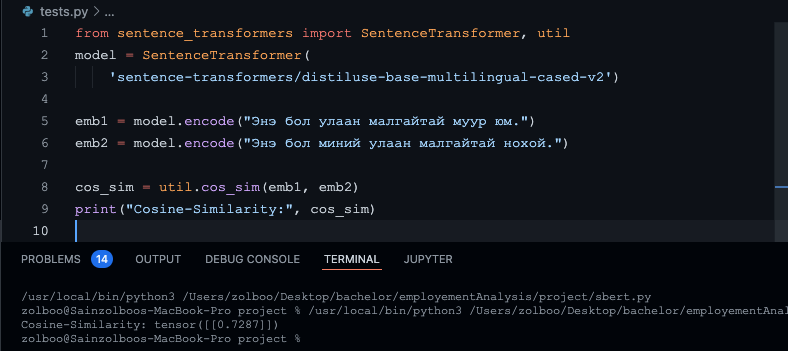
\includegraphics[width=\textwidth]{images/sbert.png}
  \caption{cosine-similarity ашигласан жишээ}\label{fig:cosineSimilarityExample}
\end{figure}
\subsection{Linear Regression - Шугаман Регресс}
Linear Regression буюу шугамар регрессийн загвар нь шулуун шугамыг ашигладаг бол логик болон шугаман бус регрессийн загвар нь муруй шугамыг ашигладаг. Шугаман регресс нь бие даасан хувьсагч хэрхэн өөрчлөгдөхийг тооцоолох боломжийг олгодог. Хоёр тоон хувьсагчийн хоорондын хамаарлыг тооцоолоход шугаман регрессийг ашигладаг бөгөөд ихэвчлэн дараах нөхцөлд ашиглагддаг. Үүнд:
\begin{itemize}
  \item Хоёр хувьсагчийн хоорондын нөлөөлөл
  \item Бие даасан хувьсагчийн тодорхой утга дахь хамааралтай хувьсагчийн утга
  \item Вариацын нэгэн төрлийн байдал
  \item Ажиглалтын бие даасан байдал
  \item Нормал байдал
\end{itemize}
\subsection{Comma Separated Values - CSV файл}
CSV нь өгөгдлийн утгуудыг тусгаарлахад таслал ашигладаг текст файл юм. Файлын мөр бүр нь өгөгдөл байдаг бөгөөд харгалзах утгуудад текст файлыг бичих энгийн өгөгдөл хадгалах технологи юм. Их өгөгдөлтэй хялбар харьцах боломжийг олгодгоороо давуу талтай.
\subsection{Microsoft Bot Framework}
\textit{Bot Framework}\footnote{https://dev.botframework.com/} нь Microsoft-ийн \textit{Azure Bot Service}-ийн тусламжтайгаар чатботыг турших, үүсгэх, удирдах, хэрэглээнд нэвтрүүлэх гэх мэт боломжуудыг нэг дор хангаж өгдөг. Энэхүү боломжуудын хүрээнд асуулт хариултыг зохицуулах, хэрэглэгчид зориулсан User Interface бүтээх, Language Understanding аргыг ашиглах гэх мэт үйлдлүүдийг хийх боломжтой.
\\Bot бүтээх үйл явцыг Azure Bot Service болон Bot Framework нь ихэд хөнгөвчилж өгдөг бөгөөд доорх зурагт үзүүлсэн дарааллын дагуу Bot системийг бүтээдэг.
\begin{figure}[ht]
  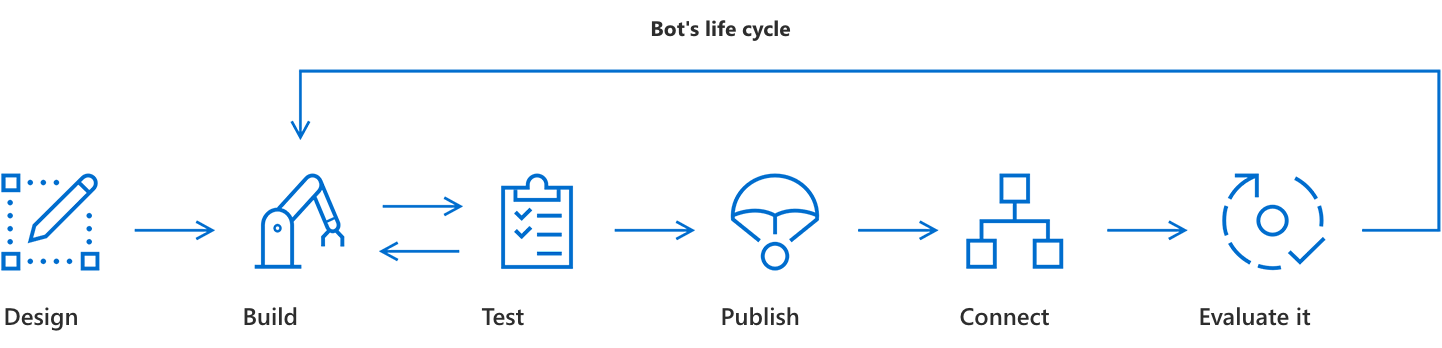
\includegraphics[width=\textwidth]{images/azureSteps.png}
  \caption{Чатботын амьралын мөчлөг}\label{fig:lifeCycle}
\end{figure}
\\\textbf{Design}
\\Design буюу загварчлах нь төслийн төлөвлөгөөг гаргах юм. Өөрөөр хэлбэл, системийн зорилго, үйл явц, хэрэглэгчийн хэрэгцээг сайтар судлах нь амжилттай Bot систем бүтээх чухал хэсэг юм.
\\\textbf{Build}
\\Бот системийг угсрах буюу хөгжүүлэх үйл явц юм. Энэ алхамд хөгжүүлэгч хэрэглэгчийн харагдах хэсгийг загварчлах бөгөөд хөгжүүлэлтийн орчин нь \textit{Azure Portal}, JavaScript, Python болон C програмчлалын хэлнүүдээс сонгож хөгжүүлэлтийг гүйцэтгэх явц юм. Мөн системийн шаардлагыг тодорхойлсны дагуу бот системийг өргөжүүлж ашиглах боломжтой бөгөөд тэдгээрээс дурдвал:
\begin{itemize}
  \item Эх хэлний боловсруулалт (NLP)
  \item Асуулт хариултыг сайжруулан мэдлэгийн сан үүсгэх
  \item Хэрэглэгчийн интерфейсийг сайжруулах
\end{itemize}
\textbf{Test}
\\Програм хангамжийн хөгжүүлэлтийн амьдралын мөчлөгийн адилаар тестийн үйл явцыг алгасаж болохгүй. Нэгэнт хэрэглэгчийн гарт бот системийг оруулахаас өмнө гарч болох алдаа дутагдлыг засан сайжруулах шаардлагатай.  Иймд Bot системийг publish хийхээс өмнө заавал туршиж үзэх шаардлагатай. Энд Microsoft-ийн өөрсдийнх нь бие даасан програм болох \textit{Bot emulator}-ийг ашиглан хөгжүүлэлтийн орчинд туршиж үзэх боломжийг олгодог. 
\\\textbf{Publish}
\\Тестийн шатны дараа бот систем ашиглахад бэлэн болсон гэж үзсэн үед төсөл эсвэл чатботыг олон нийтэд ил болгох явдал юм. 
\\\textbf{Connect}
\\Bot системээ Facebook messenger, Microsoft Teams, Telegram, Skype гэх мэт чат сувгуудыг өөрийн Bot-той холбоно.
\\Ингэж бүх мөчлөгийг дууссаны дараа хөгжүүлэгч хэрэглэгчийн ашиглаж буй байдал дээр анализ хийж системийг дахин сайжруулах боломжтой бөгөөд буцаад угсрах үйл явцруу шилжих юм. 